\section{Задача и алгоритм коллективной экспертизы}

\begin{frame}{Задача коллективной экспертизы: варианты}
 \vspace*{-3mm}
	\begin{enumerate}
		\item Методы Ю.~П.~Пытьева\footnote{Пытьев\;Ю.\,П. \emph{Эмпирическое восстановление мер возможности и правдоподобия возможности в моделях экспертных решений}, 2009}:
% .}~// Докл. АН СССР, Т.\;224, \No 6, С.\;1283--1286, 2009.\\}: 
		матрицы попарных сравнений и др.;
		\item Новый метод -- вектора предпочтений; %новый для т.\,в.~Пытьева
		\item Новый метод -- введение отношения предпорядка (частичного порядка с точностью до эквивалентности) на множестве распределений нечёткого элемента, вычислние (точной) верхней/нижней грани распределений.
	\end{enumerate} 
	
	{ \small Коллективное мнение экспертов с помощью матриц попарного сравнения: 
	\\ $\big(  \p^{(r)}(\cdot)$ -- совместное распределение на основе оценок эксперта $r = 1 \ldots R \big)$ 
	\begin{columns}
	   \column{0.5\textwidth}
	      \begin{gather*}
		   m^{(r)}_{kj} = \begin{cases}
			\;\;\;1,\;\; \p^{(r)}(t_k) > \p^{(r)}(t_j)\\
			\;\;\;0,\;\; \p^{(r)}(t_k) = \p^{(r)}(t_j)\\
			-1, \;\; \p^{(r)}(t_k) < \p^{(r)}(t_j)
		  \end{cases} 
		  \\ k,j = 1\ldots\abs{T}+1; 
		  \\ \text{причём }\p^{(r)}(t_{\abs{T}+1}) \define= 0.  
	      \end{gather*}
	   \column{0.5\textwidth}
	     \vspace*{-3mm}
	      \begin{gather*}
		  m_* = \arg \min_m \sum_{r=1}^{R} \rho(m^{(r)}, m),
		  \\ \text{где } \rho(m, m') = \big( \sum_{k,j=1}^{\abs{T}+1}(m_{kj} - {m'}_{kj})^2 \big)^{1/2}.
		  \\ \text{$m_*$ не всегда просто найти!}
	      \end{gather*}
	\end{columns}  } 
\end{frame} %===========================

\begin{frame}{Вектора предпочтений}
	\vspace{-3mm}
	{ \small Коллективное мнение экспертов с помощью векторов предпочтений аналогично случаю матриц парных сравнений ($r = 1 \ldots R$):}
	\begin{gather*}
		s^{(r)}_j = \sum_{t \in T} \mathlarger{\mathlarger{\chi} }_{A_j^{(r)}}(t),
		 \mathsmaller{\text{\small причём } \p^{(r)}(t_{\abs{T}+1}) \define= 0, \; j = 1\ldots\abs{T}+1. } 
		 \\ \text{Здесь } A^{(r)}_j = \{t \in T: \p^{(r)}(t) \leq \p^{(r)}(t_j)\}. 
	\end{gather*}
	Вектор предпочтений $s$ должен удовлетворять двум условиям:
	\\ (1) $\max s_j= |T|$ (нормировка возможности);
	\\ (2) число координат $|J_i| = i$, где $J_i = \{j: s_j \leq i\}$, $i \subset I = \{1 \ldots |T|\}$.
	
	\textbf{Задача}: $\displaystyle s_* = \arg \underset{s} \min \sum_{r=1}^R \rho(s - s^{(r)})$, где  $\displaystyle \rho(s, s') = \big( \sum_{j=1}^{\abs{T}+1}(s_{j} - {s'}_{j})^2 \big)^{1/2}$.
	
	\textbf{Алгоритм решения}:  берём  $ \ol s =  \frac{1}{R} \sum_{r=1}^R s^{(r)}$ и удовлетворяем условия (1-2), изменяя как можно меньше  координат на как можно меньшую величину.
\end{frame} %===========================

   % \begin{tikzpicture}
  %    \begin{axis}[
%	width = 0.5\textwidth, height = 0.4\textwidth,
 %   xlabel = {$L$},
%    ylabel = {$\alpha$},
	%ymin = 0, ymax = 0.4,  % if left default there will be margins
	%xmin = 2, xmax = 30,
 %   xtick = {2, 6, 10, 14, 18, 22, 26, 30}
%	xticklabels = {,,},
%	yticklabels = {,,}
%	]
%	\addplot[blue, very thick] table[x=n, y=cone] {./pic/results.txt};
%	\addplot[dash pattern=on 6pt off 3pt on 1pt off 3pt] table[x=n, y=svm] {./pic/results.txt};
%     \end{axis}
 %   \end{tikzpicture}


\begin{frame}{Предпорядок распределений возможности}
	\begin{columns}
	  \column{0.6\textwidth}
	    \begin{gather*}
	    \p_1 \prec \p_2 \text{ (читается <<уточняет>>) } \Leftrightarrow \\ 
	     \Leftrightarrow
	    \begin{cases}
 		  \supp\;p_2 \supset \supp \; \p_1;
		  \\ \exists \gamma: \p_2(\omega) = \gamma(\p_1(\omega))\;   \mathsmaller{ \omega \in \supp\;\p_1}; 
		 \\ \mathsmaller{\gamma: \zo \rightarrow \zo \text{ -- монотонная непрерывная,} } 
		%  \\ \hspace{10ex}
		\mathsmaller{\gamma(0)=0, \gamma(1)=1}
		 \\ p_2(\omega) \leq p_2(\omega'),  \mathsmaller{\omega \not\in  \supp \; \p_1,  \omega' \in  \supp \; \p_1}.
	    \end{cases}
	    \end{gather*}
	    

	    \begin{center}
		При достаточно общих условиях: %множества решений {\em задачи выбора} вложены:
		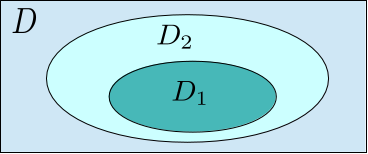
\includegraphics[width=0.75\linewidth]{./pic/solution_sets2}
		%\\ Здесь $D = 2^{\setN}$,
		\\ $\displaystyle D_r = \arg \min_d \P^{(r)}(\Eps(d))$ {\footnotesize -- решения задачи выбора на оценках $r$-го эксперта, $D$ -- все решения.}  
	     \end{center}
	  
	  \vspace*{-1mm}	   
	   {\small Оправдано использование $\p_1 \vee \p_2$ (супремума).} 
%	    \begin{gather*}
%		\mathsmaller{  \check{\p} \succ \p_1, \check{\p} \succ \p_2 }, \text{но: } \\ \forall\;\p' \neq \check{\p}, \p' \succ \p_1, \p' \succ \p_2: \p' \succ \check{\p}.
%	    \end{gather*}
	    
	%    \vspace*{2mm}
	  %  \emph{Опр.} $\hat{\p} = \p_1 \wedge \p_2$ (<<инфинум>>) -- аналогично.
	     
	%     \vspace*{1mm}

	   \column{0.4\textwidth}
	     \begin{center}
	     	\hspace*{-2mm}    \tikz{ \node (otriv){   
      \begin{tikzpicture}  \begin{axis}[width = 35mm, height = 25mm,	xticklabels = {,,}, yticklabels = {,,}, ymin = -0.1, ymax = 1.1 ]
	\addplot[green, ultra thick] table[x=xx, y=triv] {./pic/chapeter02-lattice2.dat};
       \end{axis}   \end{tikzpicture} };}
	     	    \vspace{2mm} 
		\\ \hspace*{-3mm} \tikz{ \node (osup){   
      \begin{tikzpicture}  \begin{axis}[width = 35mm, height = 25mm,	xticklabels = {,,}, yticklabels = {,,}, ymin = -0.1, ymax = 1.1 ]
	\addplot[green, very thick] table[x=xx, y=sup] {./pic/chapeter02-lattice2.dat};
       \end{axis}   \end{tikzpicture}  };}
	    \end{center} 
	     \vspace{-3mm}
	     \begin{columns}
		  \column{0.5\linewidth}
		   \begin{center}
		      \tikz{ \node (oPP1){   
      \begin{tikzpicture}  \begin{axis}[width = 35mm, height = 25mm,	xticklabels = {,,}, yticklabels = {,,}, ymin = -0.1, ymax = 1.1 ]
	\addplot[green, very thick] table[x=xx, y=pp1] {./pic/chapeter02-lattice2.dat};
       \end{axis}   \end{tikzpicture} };}
		     \vspace{-2mm}
		  \\ \tikz{ \node (oP1){   
      \begin{tikzpicture}  \begin{axis}[width = 35mm, height = 25mm,	xticklabels = {,,}, yticklabels = {,,}, ymin = -0.1, ymax = 1.1 ]
	\addplot[green, very thick] table[x=xx, y=p1] {./pic/chapeter02-lattice2.dat};
       \end{axis}   \end{tikzpicture} };}
		   \end{center} 
		  \column{0.5\linewidth}
		   \begin{center}
		     \tikz{ \node (oPP2){   
      \begin{tikzpicture}  \begin{axis}[width = 35mm, height = 25mm,	xticklabels = {,,}, yticklabels = {,,}, ymin = -0.1, ymax = 1.1 ]
	\addplot[green, very thick] table[x=xx, y=pp2] {./pic/chapeter02-lattice2.dat};
       \end{axis}   \end{tikzpicture} };}
		      \vspace{-2mm}
		  \\ \tikz{ \node (oP2){   
      \begin{tikzpicture}  \begin{axis}[width = 35mm, height = 25mm,	xticklabels = {,,}, yticklabels = {,,}, ymin = -0.1, ymax = 1.1 ]
	\addplot[green, very thick] table[x=xx, y=p2] {./pic/chapeter02-lattice2.dat};
       \end{axis}   \end{tikzpicture} };}
		   \end{center} 
	      \end{columns}
	      \begin{center}
	          \vspace{-2ex}
		 {\small  Распределения образуют полурешётку. }
	     \end{center}
	\end{columns}
	
	\begin{tikzpicture}[overlay]
		\path[->] (otriv.south) edge  (osup.north);
		\path[->] (osup.south) edge  (oPP1.north);
		\path[->] (osup.south) edge  (oPP2.north);
		\path[->] (oPP1.south) edge  (oP1.north);
		\path[->] (oPP2.south) edge  (oP2.north);
	\end{tikzpicture}	
\end{frame} %===========================



\begin{frame}{Алгоритм коллективной экспертизы}
 \begin{center}
    Пусть имеется $n$ объектов с $m$ параметрами, и $R$ экспертов, каждый из которых оценил все объекты по всем параметрам (если это не так, отсутствующие распределения считаем тривиальными.)
	\\ \vspace{3mm} \textbf{Идея}: 
	\begin{enumerate}
		\item составить <<длинные>> вектор $(\p_{11}^{(1)}, \ldots \p_{nm}^{(1)});\; (\p_{11}^{(2)}, \ldots \p_{nm}^{(2)})$ и т.\,д.;
		\item рассчитать коллективный вектор $(\p_{11}, \ldots \p_{nm})$ методом $\vee$ или методом матриц п.\,с.;
		\item Одномерные <<куски>> этого вектора, $\p_{ij}$,  считать коллективным мнением экспертов по параметрам объектов {\footnotesize $i = 1 \ldots n$, $j = 1 \ldots m$}. 
	\end{enumerate}	
 \end{center}
\end{frame} %===========================

% == eof == eof ===